
%\documentclass[11pt,a4paper,oneside]{report}
\documentclass[a4paper,12pt]{article}
\synctex=1

\usepackage{pslatex,palatino,avant,graphicx,color}
\usepackage[margin=2cm]{geometry}

\usepackage{mathptmx}       % selects Times Roman as basic font

\usepackage{helvet}         % selects Helvetica as sans-serif font
\usepackage{courier}        % selects Courier as typewriter font
\usepackage{type1cm}        % activate if the above 3 fonts are
                            % not available on your system

\usepackage{makeidx}         % allows index generation
\usepackage{graphicx}        % standard LaTeX graphics tool
                             % when including figure files
\usepackage{multicol}        % used for the two-column index
\usepackage{multirow}
\usepackage{booktabs}

\usepackage[bottom]{footmisc}% places footnotes at page bottom

\usepackage[utf8]{inputenc}
\inputencoding{utf8}

\usepackage[square,sort]{natbib}
\bibliographystyle{unsrtnat}


\usepackage[utf8]{inputenc}
\usepackage[english]{babel}

\usepackage{longtable}
\usepackage{pdflscape}

%for formula references
\usepackage{amsmath}

\newtheorem{mydef}{Definition}

\usepackage{changes}
%triangledown
\usepackage{latexsym}
\usepackage{amssymb}
\usepackage{amsfonts}
\usepackage{amsthm}

\usepackage[]{algorithm2e}

%langle
\usepackage{scalerel}
\usepackage{graphicx}


%width of the column
\usepackage{array}
\newcolumntype{L}[1]{>{\raggedright\let\newline\\\arraybackslash\hspace{0pt}}m{#1}}
\newcolumntype{C}[1]{>{\centering\let\newline\\\arraybackslash\hspace{0pt}}m{#1}}
\newcolumntype{R}[1]{>{\raggedleft\let\newline\\\arraybackslash\hspace{0pt}}m{#1}}

%rotate the name of the column
\usepackage{adjustbox}
\usepackage{array}

\newcolumntype{R}[2]{%
    >{\adjustbox{angle=#1,lap=\width-(#2)}\bgroup}%
    l%
    <{\egroup}%
}
\newcommand*\rot{\multicolumn{1}{R{90}{1em}}}% no optional argument here, please!

%checkmark
\usepackage{tikz}
\def\checkmark{\tikz\fill[scale=0.4](0,.35) -- (.25,0) -- (1,.7) -- (.25,.15) -- cycle;} 

\usepackage{setspace}


\makeindex

\begin{document}
\doublespacing

\begin{titlepage}

\begin{center}
\vspace*{-1in}
\begin{figure}[htb]
\begin{center}

\includegraphics[width=8cm]{./image/ufv1}
\end{center}
\end{figure}

CENTRO DE CIENCIAS EXATAS E TECNOLOGICAS - CCE\\
\vspace*{0.15in}
DEPARTAMENTO DE INFORMATICA \\
\vspace*{0.6in}
\begin{large}
DISSERTATION:\\
\end{large}
\vspace*{0.2in}
\begin{Large}
\textbf{ON SELECTING OF HEURISTICS FUNCTIONS FOR DOMAIN INDEPENDENT PLANNING} \\
\end{Large}
\vspace*{0.3in}
\begin{large}
%A Thesis Project submitted by Marvin Abisrror for the degree of Master to the PPG\\
\textbf{Marvin Abisrror Zarate} \\
MSc Student in Computer Science \\
\end{large}
\vspace*{0.1in}
\rule{80mm}{0.1mm}\\
\vspace*{0.1in}
\begin{large}
Levi Henrique Santana de Lelis \\
(Advisor)
\

\
Santiago Franco \\
(Co-Advisor)
\

\

\
\end{large}
VIÇOSA - MINAS GERAIS\\
MARCH - 2016
\end{center}
\end{titlepage}

\newpage

\abstract{
In this dissertation we present a greedy method based on the theory of supermodular optimization for selecting a subset of heuristics functions from a large set of heuristics with the objective of reducing the running time of the search algorithms.

 \citep{holte2006maximizing} showed that search can be faster if several smaller pattern databases are used instead of one large pattern database. We introduce a greedy method for selecting a subset of the most promising heuristicss from a large set of heuristics functions to guide the A* search algorithm. If the heuristics are consistent, our method selects a subset which is guaranteed to be near optimal with respect to the resulting A* search tree size. In addition to being consistent, if all heuristics have the same evaluation time, our subset is guaranteed to be near optimal with respect to the resulting A* running time. We implemented our method in Fast Downward and showed empirically that it produces heuristics which outperform the state of the art heuristics in the International Planning Competition benchmarks.
 
In this dissertation we advance and develop the approach of selection for solving different state-space problems. Namemly,

\begin{itemize}
  \item Develop an approach for selecting a subset of heuristic functions with the goal of reducing the running time of the search algorithms employing these functions.
  \item Develop approaches to obtain the cardinality of the subsets of heuristics found.
  \item Develop a method to find a subset of heuristics from a large pool of heuristics that optimize the number of nodes expanded in the process of search.
  \item Use Stratified Sampling (SS) algorithm for predicting the search tree size of Iterative-Deepening A* (IDA*). We use SS as our utility function. 
\end{itemize}
 
 }
\newpage

\tableofcontents

\newpage

\section{Introduction}
Every problem of Artificial Intelligent (\texttt{AI}) can be cast as a state space problem. The state space is a set of states where each state represent a possible solution to the problem and each state is linked with other states if exists a function that goes from one state to another. In the search space there are many solutions that represent the same state, each of this solutions are called node. So, many nodes can be represented as one state. To find the solution of the problem is required the use of search algorithms such as: Depth First Search (\texttt{DFS}), which looks the solution of the problem traversing the search space exploring the nodes in each branch before backtracking up to find the solution. Another search algorithm is Breadth First Search (\texttt{BFS}), which looks for the solution exploring the neighbor nodes first, before moving to the next level of neighbors. The mentioned algorithms have the characteristic that when they do the search, they generate a larger search space, basically for two main reasons: a) Consider the total number of states to be analyzed in order to determinate if the solution is found. b) There is no guide to get to the solution. The search space that these algorithms generate are called Brute force search tree (\texttt{BFST}).

There are other types of algorithms called heuristic informed search, which are algorithms that requires the use of heuristics. The heuristic is the estimation of the distance for one node in the search tree to get to the near solution. The heuristic informed search generates a smaller search tree in comparison to the \texttt{BFST}, because the heuristic guides the search exploring the nodes that are in the solution path and prunes the nodes which are not. Also, the use of heuristics reduce the running time of the search algorithm.

There are different approaches to create heuristics, such as: Pattern Databases (\texttt{PDBs}), Neural Network, and Genetic Algorithm. These systems that create heuristics receive the name of Heuristics Generators. And one of the approaches that have showed most successfull results in heuristic generation is the PDBs, which is memory-based heuristic functions obtained by abstracting away certain problem variables, so that the remaining problem ("pattern") is small enough to be solved optimally for every state by blind exhaustive search. The results stored in a table, represent a PDB for the original problem. The abstraction of the search space gives an admissible heuristic function, mapping states to lower bounds.

Exists many ways to take advantage of all the heuristics that can be created, for example: \citep{holte2006maximizing} showed that search can be faster if several smaller pattern databases are used instead of one large pattern database. In addition \citep{domshlak2010max} and \citep{tolpin2013towards} results showed that evaluating the heuristic lazily, only when they are essensial to a decision to be made in the search process is worthy in comparison to take the maximum of the set of heuristics. Then, using all the heuristics do not guarantees to solve the major number of problems in a limit time.

Finally, the objective of this dissertation is to develop meta-reasoning approaches for selecting heuristics functions from a large set of heuristics with the goal of reducing the running time of search algorithm employing these functions.

\section{Background}
A $SAS\sp{+} planning\ task$ \citep{backstrom1995complexity} is a 4 tuple $\triangledown = \{V, O, I, G\}.$ \textit{V} is a set of \textit{state variables.} Each variable \textit{v} $\in$ \textit{V} is associated with a finite domain of possible $D_{\substack{v}}$. A state is an assignment of a value to every $v \in V.$ The set of possible states, denoted \textit{V}, is therefore $D_{\substack{v_{\substack{1}}}}    \times ... \times D_{\substack{v_{\substack{2}}}}$. \textit{O} is a set of operators, where each operator $o \in O$ is triple $\{pre_{\substack{o}} , post_{\substack{o}}, cost_{\substack{o}}\}$ specifying the preconditions, postconditions (effects), and non-negative cost of \textit{o}. $pre_{\substack{o}}\ and\ post_{\substack{o}}$ are assignments of values to subsets os variables, $V_{\substack{pre_{\substack{o}}}}\ and\ V_{\substack{post_{\substack{o}}}}$, respectively. Operator \textit{o} is applicable to state \textit{s} if \textit{s} and $pre_{\substack{o}}$ agree on the assignment of values to variables in $V_{\substack{pre_{\substack{o}}}}$. The effect of \textit{o}, when applied to \textit{s}, is to set the variables in $V_{\substack{post_{\substack{o}}}}$ to the values specified in $post_{\substack{o}}$ and to set all other variables to the value they have in \textit{s}. \textit{G} is the goal condition, an assignment of values to a subset of variables, $V_{\substack{G}}$. A state is a goal state if it and \textit{G} agree on the assignment of values to the variable in $V_{\substack{G}}$. \textit{I} is the initial state, and the planning task, $\triangledown$, is to find an optimal (least-cost) sequence of operators leading from \textit{I} to a goal state. We denote the optimal solution cost of $\triangledown$ as $C\sp{*}$


The state space problem illustrated in the figure \ref{fig:8tilepuzzle} is a game that consists of a frame of numbered square tiles in random order with one tile missing. The puzzle also exists in other sizes, particularly the smaller 8$-$puzzle. If the size is 3$\times$3 tiles, the puzzle is called the 8 puzzle or 9$-$puzzle, and if 4 $\times$ 4 tiles, the puzzle is called the 15-puzzle or 16-puzzle named, respectively, for the number of tiles and the number of spaces. The object of the puzzle is to place the tiles in order by making sliding moves that use the empty space.

The legal operators are to slide any tile that is horizontally or vertically adjacent to the blank into the blank position. The problem is to rearrange the tiles from some random initial configuration into a particular desired goal configuration. The 8$-$puzzle contains 181,440 reachable states, the 15$-$puzzle contains about $10\sp{13}$ reachable states, and the 24$-$puzzle contains almost $10\sp{25}$ states.

\begin{figure}[htb]
\begin{center}
\par
\raisebox{-.2\height}{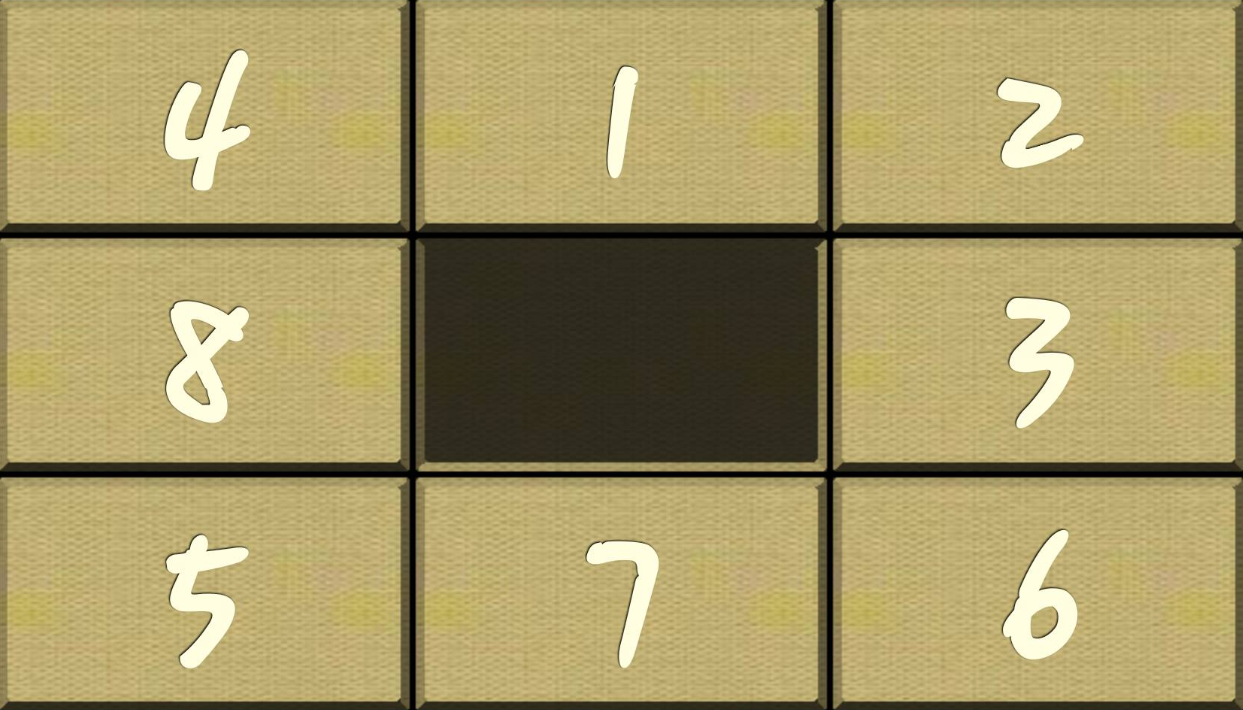
\includegraphics[width=4cm]{./image/inicio}}%
\hspace*{0.4in} %\hfill
\raisebox{-.2\height}{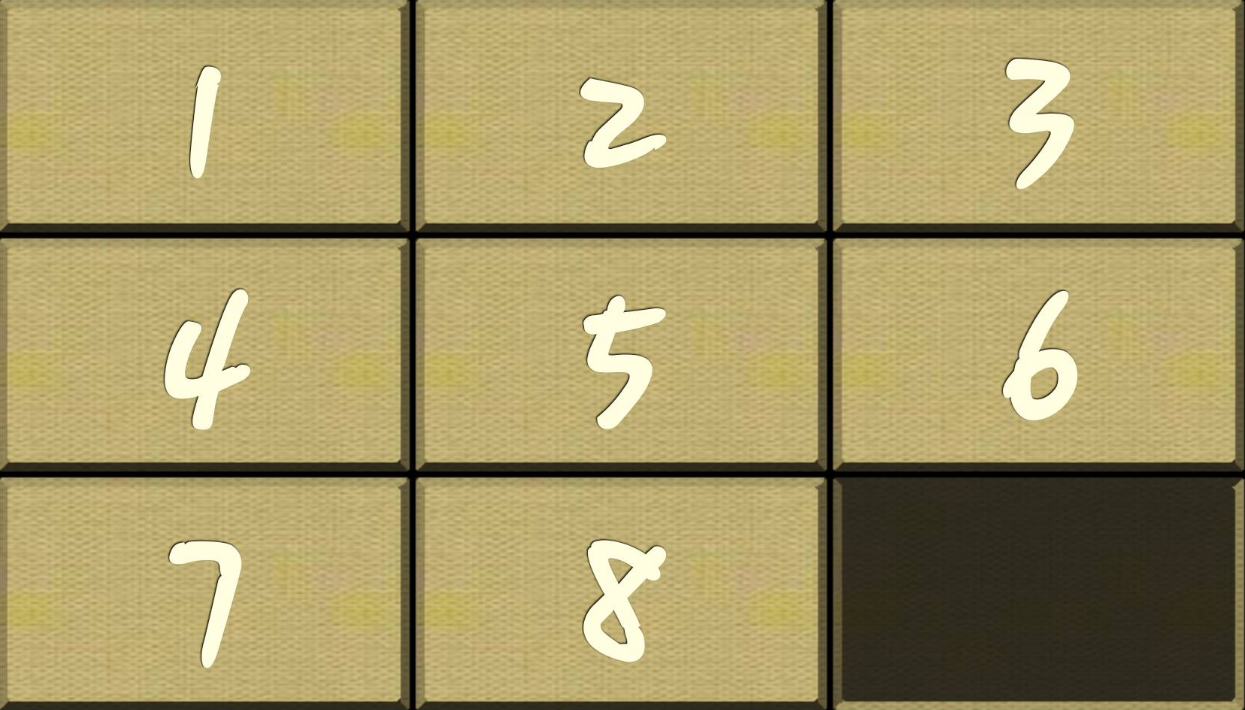
\includegraphics[width=4cm]{./image/objetivo}}%
\par
\caption{The left frame is the initial distribution of tiles and the right frame is the goal distribution of tiles.}
\label{fig:8tilepuzzle}
\end{center}
\end{figure}

\subsection{Heuristics}






Define the problem using examples


The new approach for selecting a subset of heuristics functions for domain-independent planning has two main objectives: First, make a selection of heuristics from a large set of heuristics with the goal of reducing the running time of a search algorithm employing the subset functions. Second, find out if the prediction of Stratified Sampling (SS) might be helpful in selecting a subset of heuristics to guide the A* search.

Maybe writing \citep{krause2012submodular} should demostrated something.
Cite by holte \citep{holte2006maximizing} and this.
Another cite \citep{xu2014solving} what about this.
Another cite \citep{krause2007near} what about this.
Another cite by bernand nebel \citep{backstrom1995complexity} what about this.


In order to achieve the first objective we present The Greedy Algorithm, which provides a good approximation to the optimal solution of the NP-hard optimization problem \citep{krause2012submodular}. 

In order to achieve the second objective we use the \textit{relative unsigned error} to probe the accuracy of the predictions of SS with respect to IDA*. We know that SS does not make even reasonable predictions for the number of nodes expanded by A*. Nevertheless, even though SS produces poor predictions for the number of nodes expanded by A*, we would like to verify whether these predictions can be helpful in selecting a subset of heuristics to guide the A* search.

This report have three sections, the first section is the introduction, the second is the experiment 1 which contains four main tables showing the results of the \textit{relative unsigned error}. and the last section in the conclusion.

\section{Comparison of SS with IDA*}
Stratification Sampling is an algorithm that estimates the number of nodes expanded performed by heuristic search algorithm seeking solutions in state space. We apply SS to predict the number of nodes expanded by IDA* in a given \textit{f-}layer when using a consistent heuristics.

We first ran IDA* for Fast-Downward benchmark for optimal domains. Our evaluation metric is coverage, \textit{i.e.,} number of problems solved within 24 hours time limit. We note that in 24 hours non all the instances for a specific domain using a consistent heuristic can be solved. Afterwards, run SS using as a threshold the \textit{f}-layer for each instance of each domain, this process is executed using different number of probes \textit{i.e.,} 1, 10, 100, 1000, and 5000. 

In our experiment 1, prediction accuracy is measured in terms of the \textit{Relative Unsigned Error} (ss-err), which is calculated as:


\begin{center}
$
\frac{\sum_{s\in PI} \frac{Pred(s, d) - R(s, d)}{R(s, d)}}{|PI|}
$
\end{center}

Where \textit{PI} is the set of problem instances, \textit{Pred(s, d)} and \textit{R(s, d)} are the predicted and actual number of nodes expanded by IDA* for start state \textit{s} and cost bound \textit{d}. A perfect score according to this measure is 0.000.


The heuristics used for this experiment 1 were: hmax, ipdb, lmcut, and {merge\_and\_shrink}. There are 4 tables, each table shows the results running IDA* and SS using one consistent heuristic. The first column represent the optimal domains for Fast-Downward benchmark. The remaining 10 columns shows the 5 different probes \textit{i.e.,} 1, 10, 100, 1000, and 5000. Each probe has two columns which represent the ss-err and the ss-time. The last two columns are the information for IDA* which represent the average value of the number of nodes expanded and the average time respectively. The text "---" means that IDA* could not solve the problems, consequently there are not results for SS.


\begin{table}[]
\footnotesize\setlength{\tabcolsep}{1.8pt}
\caption{Experiment 1 - Comparison using hmax heuristic}
\label{my-label}
\begin{tabular}{l@{\hspace{6pt}} *{13}{|r}}
\hline
	                                                & \multicolumn{11}{c}{hmax}                                                                                                          & \multicolumn{2}{l}{}      \\ \hline

                  & \multicolumn{2}{c|}{1} & \multicolumn{2}{c|}{10} & \multicolumn{2}{c|}{100} & \multicolumn{2}{c|}{1000} & \multicolumn{2}{c|}{5000}                   \\ \hline  
Domain                  & error  & time  & error  & time  & error  & time  & error  & time  & error  & time  & ida*  & ida*-time  & n\\ \hline
barman-opt11            & 0.60 & 0.06 & 0.45 & 0.32 & 0.20 & 3.21 & 0.07 & 32.57 & 0.04 & 214.59 & 8835990.00 & 6016.38 & 20 \\ \hline
blocks                  & 0.42 & 0.02 & 0.17 & 0.10 & 0.06 & 1.06 & 0.03 & 10.86 & 0.01 & 65.97 & 28510300.00 & 3030.97 & 35 \\ \hline
elevators-opt08         & 0.67 & 1.61 & 0.48 & 11.13 & 0.21 & 110.38 & 0.13 & 1140.05 & 0.48 & 3012.95 & 923397.00 & 4795.09 & 30 \\ \hline
elevators-opt11         & 0.84 & 1.40 & 0.42 & 9.85 & 0.23 & 96.37 & 0.13 & 994.33 & 0.14 & 4223.73 & 966309.00 & 4759.72 & 20 \\ \hline
floortile-opt11         & 2.02 & 0.01 & 0.62 & 0.07 & 0.40 & 0.69 & 0.14 & 6.93 & 0.11 & 36.60 & 30522300.00 & 3919.72 & 2 \\ \hline
nomystery-opt11         & 0.53 & 0.07 & 0.26 & 0.38 & 0.07 & 3.63 & 0.03 & 36.35 & 0.01 & 181.03 & 6565740.00 & 3256.86 & 20 \\ \hline
openstacks-adl          & --- & --- & --- & --- & --- & --- & --- & --- & --- & --- & --- & --- & --- \\ \hline
openstacks-opt08        & 0.58 & 82.20 & 0.04 & 800.37 & 0.10 & 1260.88 & 0.10 & 12368.90 & 0.22 & 9594.93 & 73087.30 & 2669.55 & 30 \\ \hline
openstacks-opt11        & 0.03 & 94.79 & 0.03 & 774.86 & 0.10 & 991.57 & 0.10 & 10148.40 & 0.24 & 8779.80 & 62942.40 & 3156.36 & 20 \\ \hline
parcprinter-opt11       & 0.00 & 0.01 & 0.00 & 0.04 & 0.00 & 0.35 & 0.00 & 3.48 & 0.00 & 17.29 & 1.00 & 0.00 & 20 \\ \hline
parking-opt11           & 0.17 & 1.79 & 0.04 & 11.36 & 0.01 & 114.28 & 0.00 & 1196.83 & 0.00 & 5835.03 & 374925.00 & 5607.50 & 20 \\ \hline
pegsol-opt11            & 0.17 & 0.01 & 0.04 & 0.04 & 0.02 & 0.37 & 0.01 & 3.69 & 0.00 & 17.88 & 68763.70 & 5.00 & 20 \\ \hline
scanalyzer-opt11        & 0.43 & 3.13 & 0.25 & 28.79 & 18.63 & 273.74 & 0.02 & 3033.06 & 0.04 & 10021.00 & 8257850.00 & 4808.75 & 20 \\ \hline
sokoban-opt08           & 0.35 & 0.27 & 0.22 & 1.95 & 0.09 & 20.24 & 0.05 & 214.01 & 0.03 & 965.40 & 2657890.00 & 3385.95 & 30 \\ \hline
sokoban-opt11           & 0.41 & 0.31 & 0.26 & 2.00 & 0.11 & 21.42 & 0.05 & 222.47 & 0.04 & 1056.61 & 3118530.00 & 3932.69 & 20 \\ \hline
tidybot-opt11           & 300.86 & 4.40 & 1072.40 & 26.48 & 5.88 & 238.76 & 0.01 & 2747.10 & 0.04 & 11572.90 & 431336.00 & 5465.62 & 20 \\ \hline
transport-opt08         & 0.55 & 0.33 & 0.36 & 2.57 & 0.27 & 23.11 & 0.13 & 236.72 & 0.10 & 1363.04 & 1462640.00 & 957.41 & 27 \\ \hline
transport-opt11         & 0.63 & 0.09 & 0.54 & 0.61 & 0.24 & 5.89 & 0.15 & 59.37 & 0.11 & 290.31 & 2622880.00 & 2253.51 & 20 \\ \hline
visitall-opt11          & 0.12 & 0.00 & 0.04 & 0.05 & 0.01 & 0.56 & 0.00 & 5.77 & 0.00 & 28.07 & 71032400.00 & 3704.78 & 20 \\ \hline
woodworking-opt08       & 0.89 & 0.16 & 0.57 & 1.44 & 0.35 & 13.94 & 0.13 & 140.83 & 0.07 & 685.86 & 4170080.00 & 4055.03 & 30 \\ \hline
woodworking-opt08       & 1.28 & 0.15 & 0.69 & 1.33 & 0.27 & 13.21 & 0.17 & 130.82 & 0.07 & 664.08 & 5139070.00 & 4944.76 & 20 \\ \hline
\end{tabular}
\end{table}


In the Table \ref{table1} we can see that there are seven domains which IDA* could not solve any instance in 24 hours. The ss-err decrease for each domain according the number of probes increases. The domains that have the perfect score are: openstacks-opt11-strips, parcprinter-opt11-strips. 

\newpage

\begin{table}[]
\footnotesize\setlength{\tabcolsep}{1.8pt}
\caption{Experiment 1 - Comparison using hmax heuristic}
\label{hmax_label}
\begin{tabular}{l@{\hspace{6pt}} *{13}{|r}}
\hline
\multicolumn{1}{c|}{} & \multicolumn{13}{c}{hmax}
\\ \hline
\multicolumn{1}{c|}{} &             &         & \multicolumn{5}{c|}{ss-error}                                                                  & \multicolumn{5}{c|}{time}                                                                                                           \\ \hline
Domain        & IDA*         & time       & 1      & 10     & 100    & 1000    & 5000       & 1      & 10     & 100    & 1000   & 50000 & n \\ \hline 
barman-opt11 & 8835990.00& 6016.38& 0.60& 0.45& 0.20& 0.07& 0.04& 0.06& 0.32& 3.21& 32.57& 214.59& 20\\ \hline
blocks & 28510300.00& 3030.97& 0.42& 0.17& 0.06& 0.03& 0.01& 0.02& 0.10& 1.06& 10.86& 65.97& 35\\ \hline
elevators-opt08 & 1628240.00& 8455.25& 0.67& 0.48& 0.21& 0.13& 0.09& 1.61& 11.13& 110.38& 1140.05& 5312.77& 30\\ \hline
elevators-opt11 & 1012570.00& 4987.57& 0.84& 0.42& 0.23& 0.13& 0.10& 1.40& 9.85& 96.37& 994.33& 4425.93& 20\\ \hline
floortile-opt11 & 30522300.00& 3919.72& 2.02& 0.62& 0.40& 0.14& 0.11& 0.01& 0.07& 0.69& 6.93& 36.60& 2\\ \hline
nomystery-opt11 & 6565740.00& 3256.86& 0.53& 0.26& 0.07& 0.03& 0.01& 0.07& 0.38& 3.63& 36.35& 181.03& 20\\ \hline
openstacks-adl & ---& ---& ---& ---& ---& ---& ---& ---& ---& ---& ---& ---& ---\\ \hline
openstacks-opt08 & 89953.60& 3285.60& 0.58& 0.04& 0.04& 0.04& 0.04& 82.20& 800.37& 1344.94& 13193.50& 11809.10& 30\\ \hline
openstacks-opt11 & 80108.50& 4017.19& 0.03& 0.03& 0.03& 0.03& 0.03& 94.79& 774.86& 1067.84& 10929.00& 11174.30& 20\\ \hline
parcprinter-opt11 & 1.00& 0.00& 0.00& 0.00& 0.00& 0.00& 0.00& 0.01& 0.04& 0.35& 3.48& 17.29& 20\\ \hline
parking-opt11 & 374925.00& 5607.50& 0.17& 0.04& 0.01& 0.00& 0.00& 1.79& 11.36& 114.28& 1196.83& 5835.03& 20\\ \hline
pegsol-opt11 & 68763.70& 5.00& 0.17& 0.04& 0.02& 0.01& 0.00& 0.01& 0.04& 0.37& 3.69& 17.88& 20\\ \hline
scanalyzer-opt11 & 8449890.00& 4920.58& 0.43& 0.25& 18.63& 0.02& 0.01& 3.13& 28.79& 273.74& 3033.06& 10254.00& 20\\ \hline
sokoban-opt08 & 2657890.00& 3385.95& 0.35& 0.22& 0.09& 0.05& 0.03& 0.27& 1.95& 20.24& 214.01& 965.40& 30\\ \hline
sokoban-opt11 & 3118530.00& 3932.69& 0.41& 0.26& 0.11& 0.05& 0.04& 0.31& 2.00& 21.42& 222.47& 1056.61& 20\\ \hline
tidybot-opt11 & 444473.00& 5632.08& 300.86& 1072.40& 5.88& 0.01& 0.01& 4.40& 26.48& 238.76& 2747.10& 11925.40& 20\\ \hline
transport-opt08 & 1462640.00& 957.41& 0.55& 0.36& 0.27& 0.13& 0.10& 0.33& 2.57& 23.11& 236.72& 1363.04& 27\\ \hline
transport-opt11 & 2622880.00& 2253.51& 0.63& 0.54& 0.24& 0.15& 0.11& 0.09& 0.61& 5.89& 59.37& 290.31& 20\\ \hline
visitall-opt11 & 71032400.00& 3704.78& 0.12& 0.04& 0.01& 0.00& 0.00& 0.00& 0.05& 0.56& 5.77& 28.07& 20\\ \hline
woodworking-opt08 & 4170080.00& 4055.03& 0.89& 0.57& 0.35& 0.13& 0.07& 0.16& 1.44& 13.94& 140.83& 685.86& 30\\ \hline
woodworking-opt08 & 5139070.00& 4944.76& 1.28& 0.69& 0.27& 0.17& 0.07& 0.15& 1.33& 13.21& 130.82& 664.08& 20\\ \hline
\end{tabular}
\end{table}

\begin{table}[]
\centering
\caption{Poor prediction of SS against A* ipdb}
\label{my-label}
\begin{tabular}{l|l|l|l}
\hline
\multicolumn{4}{l}{Experiment 2: Using ipdb heuristic - 500 in gapdb\_deep} \\ \hline
Domain& A*& ss error& n \\ \hline

blocks& 2.07455e+06& 9.20794e+31& 18\\ \hline
barman-opt11-strips& 1.71877e+07& 5.84137e+32& 4\\ \hline
elevators-opt08-strips& 1.39911e+07& 9.2879e+23& 7\\ \hline
elevators-opt11-strips& 1.83142e+07& 1.3003e+24& 5\\ \hline
floortile-opt11-strips& 1.40015e+07& 7.52158e+16& 4\\ \hline
nomystery-opt11-strips& 40169.7& 1.15599e+34& 9\\ \hline
openstacks-opt08-strips& 1874.5& 999720& 2\\ \hline
parcprinter-opt11-strips& 1157& 2.56184e+22& 3\\ \hline
scanalyzer-opt11-strips& 337894& 3.71451e+32& 3\\ \hline
sokoban-opt08-strips& 1136.25& 3.48709e+08& 4\\ \hline
sokoban-opt11-strips& 861& 0.938381& 1\\ \hline
transport-opt08-strips& 755974& 1.90383e+39& 5\\ \hline
transport-opt11-strips& 1.88894e+06& 2.91167e+38& 2\\ \hline
visitall-opt11-strips& 8.12101e+06& 3.18043e+43& 8\\ \hline
woodworking-opt08-strips& 1.50059e+06& 8.65693e+17& 7\\ \hline
woodworking-opt11-strips& 4.81226e+06& 3.02819e+18& 2\\ \hline
\end{tabular}
\end{table}


\begin{table}[]
\centering
\caption{Poor prediction of SS against A* lmcut}
\label{my-label}
\begin{tabular}{l|l|l|l}
\hline
\multicolumn{4}{l}{Experiment 2: Using lmcut heuristic - 500 in gapdb\_deep} \\ \hline
Domain& A*& ss error& n \\ \hline

blocks& 2.39089e+06& 2.68279e+31& 18\\ \hline
barman-opt11-strips& 7.44986e+06& 9.16154e+28& 4\\ \hline
elevators-opt08-strips& 1.17502e+07& 3.7338e+19& 7\\ \hline
elevators-opt11-strips& 1.5278e+07& 5.22719e+19& 5\\ \hline
floortile-opt11-strips& 702435& 6.21105e+10& 4\\ \hline
nomystery-opt11-strips& 267100& 1.03783e+26& 9\\ \hline
openstacks-opt08-strips& 1874.5& 953648& 2\\ \hline
parcprinter-opt11-strips& 1363.67& 2.33125e+21& 3\\ \hline
scanalyzer-opt11-strips& 334747& 7.55436e+30& 3\\ \hline
sokoban-opt08-strips& 1000.75& 2.27145e+08& 4\\ \hline
sokoban-opt11-strips& 861& 0.938381& 1\\ \hline
transport-opt08-strips& 594665& 4.60306e+24& 5\\ \hline
transport-opt11-strips& 1.48569e+06& 1.15083e+25& 2\\ \hline
visitall-opt11-strips& 8.1205e+06& 3.18043e+43& 8\\ \hline
woodworking-opt08-strips& 1.49993e+06& 9.17535e+17& 7\\ \hline
woodworking-opt11-strips& 4.81236e+06& 3.2025e+18& 2\\ \hline
\end{tabular}
\end{table}

\begin{table}[]
\centering
\caption{Poor prediction of SS against A* mands}
\label{my-label}
\begin{tabular}{l|l|l|l}
\hline
\multicolumn{4}{l}{Experiment 2: Using mands heuristic - 500 in gapdb\_deep} \\ \hline
Domain& A*& ss error& n \\ \hline

blocks& 2.96963e+06& 1.01528e+31& 18\\ \hline
barman-opt11-strips& 2.67042e+07& 2.08212e+36& 4\\ \hline
elevators-opt08-strips& 1.58876e+07& 6.50833e+26& 7\\ \hline
elevators-opt11-strips& 2.0719e+07& 9.11162e+26& 5\\ \hline
floortile-opt11-strips& 3.26068e+07& 7.36763e+16& 4\\ \hline
nomystery-opt11-strips& 8236& 2.02873e+26& 9\\ \hline
openstacks-opt08-strips& 1874.5& 299017& 2\\ \hline
parcprinter-opt11-strips& 766.333& 6.35555e+20& 3\\ \hline
scanalyzer-opt11-strips& 337893& 1.76874e+29& 3\\ \hline
sokoban-opt08-strips& 602.5& 4.08107e+08& 4\\ \hline
sokoban-opt11-strips& 861& 0.938381& 1\\ \hline
transport-opt08-strips& 741293& 2.72958e+37& 5\\ \hline
transport-opt11-strips& 1.85225e+06& 6.82396e+37& 2\\ \hline
visitall-opt11-strips& 8.121e+06& 3.22741e+43& 8\\ \hline
woodworking-opt08-strips& 5.48249e+06& 1.21766e+18& 7\\ \hline
woodworking-opt11-strips& 1.77967e+07& 4.26012e+18& 2\\ \hline
\end{tabular}
\end{table}


%below of this is commenting everything

\iffalse

\begin{table}[]
\footnotesize\setlength{\tabcolsep}{2.0pt}
\caption{ss-err variation}
\label{subTable1}
\begin{tabular}{l@{\hspace{6pt}} *{12}{c}}
\hline
                        & \multicolumn{2}{c|}{1} & \multicolumn{2}{c|}{10} & \multicolumn{2}{c|}{100} & \multicolumn{2}{c|}{1000} & \multicolumn{2}{c|}{5000} &            &          \\ \hline
Domain                  & ss-err        & ss-t   & ss-err        & ss-t    & ss-err        & ss-t     & ss-err        & ss-t      & ss-err        & ss-t      & ida*       & ida-time \\ \hline
openstacks-opt08-strips & {\bf 0.192}   & 0.668  & {\bf 0.141}   & 6.636   & {\bf 0.128}   & 67.228   & {\bf 0.141}   & 679.132   & {\bf 0.146}   & 3365.820  & 361346.000 & 786.512  \\ \hline
\end{tabular}
\end{table}

In the Table \ref{subTable1} the ss-err with 1 probe is \textbf{0.192}, afterwards it descrease with 10 probes to \textbf{0.141}, afterwards it decrease to \textbf{0.128}, but with 1000 probes instead to continue decreasing the opposite happens, it increase to \textbf{0.141} and continue increasing using 5000 probes to \textbf{0.146}. This kind of results might be due the fact that SS can consider more predictions and that some of them increase the result of the ss-err.

\newpage

\begin{table}[]
\footnotesize\setlength{\tabcolsep}{1.0pt}
\caption{Experiment 1 - Comparison using ipdb heuristic}
\label{table2}
\begin{tabular}{l@{\hspace{4pt}} *{12}{c}}
\hline
                                                        & \multicolumn{10}{c}{ipdb}                                                                                                          & \multicolumn{2}{l}{}      \\ \hline

                  & \multicolumn{2}{|c|}{1} & \multicolumn{2}{c|}{10} & \multicolumn{2}{c|}{100} & \multicolumn{2}{c|}{1000} & \multicolumn{2}{c|}{5000}                   \\ \hline
Domain                  & ss-err  & ss-t  & ss-err  & ss-t  & ss-err  & ss-t  & ss-err  & ss-t  & ss-err  & ss-t  & ida*  & ida-time  \\ \hline
barman-opt11-strips     & --- & --- & --- & --- & --- & --- & --- & --- & --- & --- & --- & --- \\ \hline
blocks                  & 4.789 & 0.002 & 3.543 & 0.013 & 1.678 & 0.134 & 0.742 & 1.366 & 0.485 & 6.909 & 2096930000.000 & 10018.200 \\ \hline
elevators-opt08-strips  & 8.909 & 0.835 & 5.724 & 8.550 & 4.030 & 85.280 & 1.583 & 858.460 & 1.183 & 4287.430 & 95651000.000 & 20223.900 \\ \hline
elevators-opt11-strips  & 13.495 & 1.130 & 9.043 & 11.380 & 3.898 & 117.380 & 2.846 & 1178.090 & 1.771 & 5904.640 & 154128000.000 & 36205.900 \\ \hline
floortile-opt11-strips  & --- & --- & --- & --- & --- & --- & --- & --- & --- & --- & --- & --- \\ \hline
nomystery-opt11-strips  & 1429.530 & 0.003 & 1.759 & 0.011 & 1.065 & 0.114 & 0.475 & 1.103 & 0.167 & 5.536 & 360878000.000 & 2514.160 \\ \hline
openstacks-opt08-adl    & --- & --- & --- & --- & --- & --- & --- & --- & --- & --- & --- & --- \\ \hline
openstacks-opt08-strips & 0.376 & 0.820 & 0.301 & 7.631 & 0.279 & 75.666 & 0.293 & 772.126 & 0.290 & 4522.480 & 2043600.000 & 15633.000 \\ \hline
openstacks-opt11-strips & 0.316 & 1.827 & 0.449 & 16.107 & 0.457 & 172.507 & 0.442 & 1678.330 & 0.437 & 9491.130 & 4166230.000 & 35539.000 \\ \hline
parcprinter-opt11-strips& 0.040 & 0.000 & 0.011 & 0.006 & 0.006 & 0.071 & 0.000 & 0.735 & 0.077 & 3.603 & 3065.690 & 337.491 \\ \hline
parking-opt11-strips    & 3.584 & 0.028 & 1.488 & 0.200 & 0.399 & 2.116 & 0.135 & 20.748 & 0.288 & 103.608 & 306957000.000 & 7448.660 \\ \hline
pegsol-opt11-strips     & 1.515 & 0.047 & 0.662 & 0.387 & 0.342 & 3.973 & 0.327 & 39.435 & 0.376 & 190.308 & 54945.300 & 1181.480 \\ \hline
scanalyzer-opt11-strips & 1.353 & 0.003 & 49.072 & 0.097 & 0.167 & 0.857 & 0.342 & 8.326 & 0.036 & 42.423 & 1071520000.000 & 8163.320 \\ \hline
sokoban-opt08-strips    & 0.112 & 0.006 & 0.026 & 0.035 & 0.005 & 0.372 & 0.004 & 3.654 & 0.003 & 18.271 & 280429.000 & 9.525 \\ \hline
sokoban-opt11-strips    & 0.073 & 0.007 & 0.001 & 0.049 & 0.004 & 0.482 & 0.002 & 4.869 & 0.001 & 24.387 & 404338.000 & 13.458 \\ \hline
tidybot-opt11-strips    & 1.759 & 0.080 & 0.637 & 0.853 & 0.416 & 8.400 & 0.096 & 84.127 & 0.036 & 420.853 & 1131220.000 & 355.400 \\ \hline
transport-opt08-strips  & 0.000 & 0.000 & 0.000 & 0.000 & 0.000 & 0.000 & 0.000 & 0.040 & 0.000 & 0.260 & 15.000 & 0.120 \\ \hline
transport-opt11-strips  & --- & --- & --- & --- & --- & --- & --- & --- & --- & --- & --- & --- \\ \hline
visitall-opt11-strips   & 1.136 & 0.002 & 0.784 & 0.015 & 0.234 & 0.080 & 0.075 & 0.840 & 0.055 & 3.989 & 7604630.000 & 31.693 \\ \hline
woodworking-opt08-strips& 2.541 & 0.037 & 0.950 & 0.287 & 0.384 & 2.817 & 0.092 & 27.843 & 0.054 & 138.885 & 93740200.000 & 6484.690 \\ \hline
woodworking-opt11-strips& 3.093 & 0.060 & 1.808 & 0.573 & 0.354 & 5.913 & 0.248 & 59.680 & 0.116 & 295.787 & 249863000.000 & 16954.900 \\ \hline
\end{tabular}
\end{table}

In Table \ref{table2} we can see that there are four domains which IDA* could not solve any instance in 24 hours. The ss-err decrease for most of the domains domain according the number of probes increases. There are few exception for example the domain parcrinter-opt11-strips that have the following result:

\begin{table}[]
\footnotesize\setlength{\tabcolsep}{2.4pt}
\caption{ss-err variation}
\label{subTable2}
\begin{tabular}{l@{\hspace{6pt}} *{12}{c}}
\hline
                         & \multicolumn{2}{|c|}{1} & \multicolumn{2}{c|}{10} & \multicolumn{2}{c|}{100} & \multicolumn{2}{c|}{1000} & \multicolumn{2}{c|}{5000} &          &          \\ \hline
Domain                   & ss-err     & ss-t      & ss-err      & ss-t      & ss-err      & ss-t       & ss-err       & ss-t       & ss-err       & ss-t       & ida*     & ida-time \\ \hline
parcprinter-opt11-strips & \textbf{0.040}      & 0.000     & \textbf{0.011}       & 0.006     & \textbf{0.006}       & 0.071      & \textbf{0.000}        & 0.735      & \textbf{0.077}        & 3.603      & 3065.690 & 337.491  \\ \hline
\end{tabular}
\end{table}

In the Table \ref{subTable2} the perfect score is found in the probe 1000. In the probe 5000 the ss-err change to 0.077. The true is that there are not better number than the perfect score. When SS is run using 5000 probes is possible that exists quite changes in the results that increase the result of the ss-err.
\newpage

\begin{table}[]
\footnotesize\setlength{\tabcolsep}{0.2pt}
\caption{Experiment 1 - Comparison using lmcut heuristic}
\label{table3}
\begin{tabular}{l@{\hspace{2pt}} *{12}{c}}
\hline
                                                        & \multicolumn{10}{c}{lmcut}                                                                                                          & \multicolumn{2}{l}{}      \\ \hline

                  & \multicolumn{2}{|c|}{1} & \multicolumn{2}{c|}{10} & \multicolumn{2}{c|}{100} & \multicolumn{2}{c|}{1000} & \multicolumn{2}{c|}{5000}                   \\ \hline
Domain                  & ss-err  & ss-t  & ss-err  & ss-t  & ss-err  & ss-t  & ss-err  & ss-t  & ss-err  & ss-t  & ida*  & ida-time  \\ \hline
barman-opt11-strips     & --- & --- & --- & --- & --- & --- & --- & --- & --- & --- & --- & --- \\ \hline
blocks                  & 3.266 & 0.164 & 2.120 & 1.667 & 0.708 & 15.701 & 0.290 & 157.335 & 0.174 & 801.386 & 9943800.000 & 9361.030 \\ \hline
elevators-opt08-strips  & 5.720 & 70.105 & 3.457 & 691.590 & 0.911 & 6210.870 & 0.299 & 61445.500 & 0.242 & 323240.000 & 139417.000 & 1458.650 \\ \hline
elevators-opt11-strips  & 6.570 & 117.520 & 4.427 & 1190.320 & 1.717 & 10650.500 & 0.642 & 107014.000 & 0.310 & 577514.000 & 220608.000 & 2573.950 \\ \hline
floortile-opt11-strips  & 12.185 & 1.340 & 3.174 & 14.740 & 2.227 & 132.460 & 0.450 & 1311.420 & 0.256 & 7195.940 & 25413400.000 & 21021.000 \\ \hline
nomystery-opt11-strips  & 4.515 & 1.262 & 1.490 & 14.763 & 0.675 & 124.755 & 0.204 & 1262.320 & 0.144 & 6858.100 & 647051.000 & 5214.300 \\ \hline
openstacks-opt08-adl    & --- & --- & --- & --- & --- & --- & --- & --- & --- & --- & --- & --- \\ \hline
openstacks-opt08-strips & 0.092 & 0.544 & 0.157 & 5.972 & 0.148 & 58.472 & 0.140 & 576.712 & 0.147 & 3911.320 & 361346.000 & 677.368 \\ \hline
openstacks-opt11-strips & 0.000 & 1.060 & 0.000 & 10.300 & 0.000 & 66.780 & 0.000 & 672.900 & 0.000 & 3698.520 & 195.000 & 2.320 \\ \hline
parcprinter-opt11-strips& 0.005 & 0.038 & 0.006 & 0.362 & 0.000 & 3.558 & 0.000 & 36.046 & 0.000 & 182.945 & 3064.850 & 0.045 \\ \hline
parking-opt11-strips    & 1.869 & 7.060 & 0.992 & 75.100 & 0.210 & 732.120 & 0.211 & 7424.720 & 0.177 & 38761.900 & 286812.000 & 4761.780 \\ \hline
pegsol-opt11-strips     & 21.763 & 0.098 & 0.373 & 0.868 & 0.240 & 7.798 & 0.213 & 74.579 & 0.159 & 393.330 & 1130870.000 & 630.318 \\ \hline
scanalyzer-opt11-strips & 1.112 & 13.417 & 0.383 & 128.737 & 0.094 & 1176.560 & 0.039 & 11800.200 & 0.024 & 76516.400 & 7211710.000 & 12482.300 \\ \hline
sokoban-opt08-strips    & 0.028 & 0.527 & 0.038 & 5.053 & 0.003 & 50.950 & 0.003 & 507.744 & 0.001 & 2915.320 & 232738.000 & 287.884 \\ \hline
sokoban-opt11-strips    & 0.038 & 0.678 & 0.005 & 6.507 & 0.004 & 63.178 & 0.002 & 633.602 & 0.001 & 3260.390 & 295998.000 & 368.898 \\ \hline
tidybot-opt11-strips    & 4.918 & 19.740 & 1.818 & 186.110 & 0.685 & 1788.940 & 0.280 & 17720.700 & 0.159 & 95541.000 & 1162760.000 & 17561.200 \\ \hline
transport-opt08-strips  & 4.542 & 0.360 & 1.012 & 3.993 & 0.392 & 38.387 & 0.125 & 384.567 & 0.049 & 2069.430 & 712491.000 & 778.980 \\ \hline
transport-opt11-strips  & --- & --- & --- & --- & --- & --- & --- & --- & --- & --- & --- & --- \\ \hline
visitall-opt11-strips   & 1.441 & 0.022 & 3.187 & 0.456 & 0.175 & 4.473 & 0.066 & 46.993 & 0.048 & 237.667 & 595466.000 & 91.538 \\ \hline
woodworking-opt08-strips& 1.123 & 0.211 & 0.266 & 1.854 & 0.148 & 18.497 & 0.019 & 188.931 & 0.029 & 1051.260 & 6048240.000 & 1859.450 \\ \hline
woodworking-opt11-strips& 0.789 & 0.320 & 0.131 & 3.490 & 0.228 & 32.830 & 0.063 & 322.000 & 0.013 & 1654.180 & 21020800.000 & 6462.270 \\ \hline
\end{tabular}
\end{table}

In the Table \ref{table3} we can see that there are three domains which IDA* could not solve any instance in 24 hours. The ss-err decrease for most of the domains according the number of probes increases, except for openstacks-opt08-strips, parcprinter-opt11-strips, sokoban-opt08-strips, visitall-opt11-strips. Nevertheless, the decrease is not a pattern, it means that only occur between two consecutive probes and the difference is minimal. The domains that have the perfect score are: openstacks-opt11-strips and parcprinter-opt11-strips.

\newpage

\begin{table}[]
\footnotesize\setlength{\tabcolsep}{1.0pt}
\caption{Experiment 1 - Comparison using {merge\_and\_shrink} heuristic}
\label{table4}
\begin{tabular}{l@{\hspace{4pt}} *{12}{c}}
\hline
                                      & \multicolumn{10}{c}{{merge\_and\_shrink}}                                                                                                          & \multicolumn{2}{l}{}      \\ \hline

                  & \multicolumn{2}{|c|}{1} & \multicolumn{2}{c|}{10} & \multicolumn{2}{c|}{100} & \multicolumn{2}{c|}{1000} & \multicolumn{2}{c|}{5000}                   \\ \hline
Domain                  & ss-err  & ss-t  & ss-err  & ss-t  & ss-err  & ss-t  & ss-err  & ss-t  & ss-err  & ss-t  & ida*  & ida-time  \\ \hline
barman-opt11-strips     & --- & --- & --- & --- & --- & --- & --- & --- & --- & --- & --- & --- \\ \hline
blocks                  & 2.163 & 13.074 & 3.346 & 13.444 & 0.482 & 14.151 & 0.205 & 14.769 & 0.256 & 17.972 & 5807970.000 & 75.288 \\ \hline
elevators-opt08-strips  & 2.479 & 4.690 & 1.968 & 7.370 & 1.293 & 34.820 & 0.970 & 292.250 & 0.924 & 1440.010 & 69178500.000 & 14434.600 \\ \hline
elevators-opt11-strips  & --- & --- & --- & --- & --- & --- & --- & --- & --- & --- & --- & --- \\ \hline
floortile-opt11-strips  & --- & --- & --- & --- & --- & --- & --- & --- & --- & --- & --- & --- \\ \hline
nomystery-opt11-strips  & 0.766 & 0.861 & 0.453 & 0.866 & 0.289 & 1.027 & 0.194 & 1.374 & 0.212 & 3.366 & 800639000.000 & 3766.920 \\ \hline
openstacks-opt08-adl    & --- & --- & --- & --- & --- & --- & --- & --- & --- & --- & --- & --- \\ \hline
openstacks-opt08-strips & 0.666 & 37.090 & 0.518 & 26.655 & 0.182 & 54.095 & 0.175 & 180.090 & 0.181 & 838.820 & 451632.000 & 358.620 \\ \hline
openstacks-opt11-strips & --- & --- & --- & --- & --- & --- & --- & --- & --- & --- & --- & --- \\ \hline
parcprinter-opt11-strips& 0.055 & 16.812 & 0.008 & 17.260 & 0.005 & 16.925 & 0.001 & 17.323 & 0.000 & 17.846 & 3064.850 & 16.872 \\ \hline
parking-opt11-strips    & --- & --- & --- & --- & --- & --- & --- & --- & --- & --- & --- & --- \\ \hline
pegsol-opt11-strips     & --- & --- & --- & --- & --- & --- & --- & --- & --- & --- & --- & --- \\ \hline
scanalyzer-opt11-strips & --- & --- & --- & --- & --- & --- & --- & --- & --- & --- & --- & --- \\ \hline
sokoban-opt08-strips    & 0.039 & 59.195 & 0.011 & 56.500 & 0.000 & 75.720 & 0.000 & 67.545 & 0.000 & 116.690 & 4135.000 & 57.275 \\ \hline
sokoban-opt11-strips    & 0.000 & 235.760 & 0.000 & 267.320 & 0.000 & 371.140 & 0.000 & 318.020 & 0.000 & 458.180 & 5.000 & 223.340 \\ \hline
tidybot-opt11-strips    & 0.000 & 1211.100 & 1.000 & 0.000 & 0.000 & 1206.820 & 0.000 & 1592.380 & 0.000 & 1326.720 & 65.000 & 1823.720 \\ \hline
transport-opt08-strips  & 0.139 & 0.016 & 0.025 & 0.020 & 0.004 & 0.044 & 0.003 & 0.172 & 0.004 & 0.804 & 1391.800 & 0.024 \\ \hline
transport-opt11-strips  & --- & --- & --- & --- & --- & --- & --- & --- & --- & --- & --- & --- \\ \hline
visitall-opt11-strips   & 0.533 & 0.818 & 0.416 & 0.902 & 0.180 & 0.907 & 0.036 & 1.058 & 0.019 & 2.318 & 2613370.000 & 9.673 \\ \hline
woodworking-opt08-strips& 0.707 & 9.966 & 0.400 & 11.906 & 0.137 & 11.640 & 0.041 & 17.886 & 0.025 & 47.763 & 10699200.000 & 303.166 \\ \hline
woodworking-opt11-strips& 1.686 & 32.360 & 1.761 & 35.480 & 0.221 & 43.670 & 0.062 & 58.410 & 0.690 & 113.240 & 36373700.000 & 1057.370 \\ \hline
\end{tabular}
\end{table}

In the Table \ref{table4} we can see that there are nine domains which IDA* could not solve any instance in 24 hours. The ss-err decrease for each domain according the number of probes increases. The domains that have the perfect score are: parcprinter-opt11-strips, sokoban-opt08-strips, sokoban-opt11-strips, and tidybot-opt11-strips.

\newpage
\section{Conclusions}
The Table \ref{table4} using {merge\_and\_shrink} has more unsolved domains and one of the reason why this happen is because it throws run out memory for most of the problems. However, is the same Table \ref{table4} which contains more perfect scores and the reason could be that {merge\_and\_shrink} generates more precise pattern database when it initializes and give us better heuristics to guide the search. The Table \ref{table3} shows that the heuristic lmcut solved most of the domains in  24 hours, which implies that lmcut give us better heuristics too. The domains that could not be solved by all the consistent heuristic were openstacks-opt08-adl, barman-opt11-strips, and transport-opt11-strips. The problem of openstacks-opt08-adl is that do not support axioms and the other domains contains difficult instances that were not possible to solve any instance within 24 hours.\\

Generally, the ss-err decreases for the most part of the domains when the number of probes increases. I think SS gives us good predictions for IDA*.

\begin{table}[]
\footnotesize\setlength{\tabcolsep}{1.8pt}
\caption{Experiment 1 - Comparison using hmax heuristic}
\label{my-label}
\begin{tabular}{l@{\hspace{6pt}} *{13}{|r}}
\hline
                                                        & \multicolumn{11}{c}{hmax}                                                                                                          & \multicolumn{2}{l}{}      \\ \hline

                  & \multicolumn{2}{c|}{1} & \multicolumn{2}{c|}{10} & \multicolumn{2}{c|}{100} & \multicolumn{2}{c|}{1000} & \multicolumn{2}{c|}{5000}                   \\ \hline
Domain                  & error  & time  & error  & time  & error  & time  & error  & time  & error  & time  & ida*  & ida*-time  & n\\ \hline
barman-opt11            & --- & --- & --- & --- & --- & --- & --- & --- & --- & --- & --- & --- & --- \\ \hline
blocks                  & 2.65 & 0.00 & 1.11 & 0.18 & 0.50 & 2.27 & 0.16 & 23.30 & 0.09 & 116.33 & 156474000.00 & 10770.90 & 13 \\ \hline
elevators-opt08         & 5.53 & 7.32 & 4.82 & 75.70 & 1.79 & 739.50 & 1.78 & 7571.86 & 1.55 & 37949.90 & 1604640.00 & 4358.74 & 1 \\ \hline
elevators-opt11         & --- & --- & --- & --- & --- & --- & --- & --- & --- & --- & --- & --- & --- \\ \hline
floortile-opt11         & --- & --- & --- & --- & --- & --- & --- & --- & --- & --- & --- & --- & --- \\ \hline
nomystery-opt11         & 9.20 & 0.04 & 2.47 & 0.36 & 0.74 & 3.71 & 0.37 & 36.85 & 0.13 & 183.90 & 2911010.00 & 289.45 & 6 \\ \hline
openstacks-adl          & --- & --- & --- & --- & --- & --- & --- & --- & --- & --- & --- & --- & --- \\ \hline
openstacks-opt08        & 0.19 & 0.67 & 0.14 & 6.64 & 0.13 & 67.23 & 0.14 & 679.13 & 0.15 & 3365.82 & 361346.00 & 786.51 & 5 \\ \hline
openstacks-opt11        & 0.00 & 0.86 & 0.00 & 8.30 & 0.00 & 80.40 & 0.00 & 798.20 & 0.00 & 4196.76 & 195.00 & 2.56 & 1 \\ \hline
parcprinter-opt11       & 0.00 & 0.00 & 0.00 & 0.04 & 0.00 & 0.39 & 0.00 & 3.34 & 0.00 & 17.29 & 1.00 & 0.00 & 20 \\ \hline
parking-opt11           & --- & --- & --- & --- & --- & --- & --- & --- & --- & --- & --- & --- & --- \\ \hline
pegsol-opt11            & 0.29 & 0.01 & 0.11 & 0.08 & 0.03 & 0.85 & 0.03 & 7.93 & 0.01 & 39.33 & 151280.00 & 11.00 & 20 \\ \hline
scanalyzer-opt11        & 0.96 & 0.08 & 0.18 & 0.12 & 0.12 & 0.88 & 0.03 & 8.08 & 0.02 & 39.92 & 101.00 & 0.16 & 1 \\ \hline
sokoban-opt08           & 0.11 & 0.04 & 0.31 & 0.35 & 0.29 & 3.52 & 0.02 & 30.99 & 0.02 & 155.11 & 5545.65 & 1.81 & 20 \\ \hline
sokoban-opt11           & 1.80 & 0.04 & 0.14 & 0.33 & 0.12 & 3.32 & 0.02 & 33.01 & 0.01 & 162.38 & 8245.92 & 2.62 & 13 \\ \hline
tidybot-opt11           & 3.75 & 5.73 & 1.58 & 29.97 & 0.61 & 287.37 & 0.27 & 2843.17 & 0.19 & 15769.20 & 2716460.00 & 17900.10 & 3 \\ \hline
transport-opt08         & 0.62 & 0.00 & 0.22 & 0.00 & 0.02 & 0.04 & 0.02 & 0.80 & 0.01 & 4.08 & 38.00 & 0.00 & 1 \\ \hline
transport-opt11         & --- & --- & --- & --- & --- & --- & --- & --- & --- & --- & --- & --- & --- \\ \hline
visitall-opt11          & 0.45 & 0.00 & 0.19 & 0.00 & 0.07 & 0.28 & 0.02 & 3.20 & 0.02 & 16.25 & 5363080.00 & 96.12 & 7 \\ \hline
woodworking-opt08       & 7.06 & 0.10 & 5.48 & 1.25 & 1.70 & 12.90 & 0.53 & 129.28 & 0.35 & 646.35 & 5190350.00 & 1023.72 & 4 \\ \hline
woodworking-opt08       & --- & --- & --- & --- & --- & --- & --- & --- & --- & --- & --- & --- & --- \\ \hline
\end{tabular}
\end{table}

\fi


\newpage
%Imports the bibliography file "references.bib"
\bibliography{references}
%\bibliographystyle{references}

\end{document}
